\documentclass[11pt,a4paper,fontset=none]{ctexart}
\usepackage[margin=1in]{geometry}
\usepackage{fontspec}
% Latin: Times New Roman (Mac / Windows) or TeX Gyre Termes (Linux); CJK: Songti / Heiti (Mac) or Fandol by file name
\IfFontExistsTF{Times New Roman}{\setmainfont{Times New Roman}}{\setmainfont{TeX Gyre Termes}}
\IfFontExistsTF{Songti SC}{%
  \setCJKmainfont{Songti SC}[BoldFont={Songti SC Bold}]%
  \setCJKsansfont{Heiti SC}\setCJKmonofont{Heiti SC}}{%
  \setCJKmainfont{FandolSong-Regular.otf}[BoldFont=FandolSong-Bold.otf]%
  \setCJKsansfont{FandolHei-Regular.otf}[BoldFont=FandolHei-Bold.otf]\setCJKmonofont{FandolHei-Regular.otf}}
\usepackage{amsmath,amssymb}
\usepackage{booktabs,array,multirow,makecell,tabularx,longtable}
\usepackage{graphicx,float,adjustbox,placeins}
\usepackage[table]{xcolor}
\usepackage[font=small,labelfont=bf,labelsep=quad]{caption}
\usepackage{enumitem}
\usepackage[numbers,square,sort&compress]{natbib}
\usepackage{xurl}
\usepackage[colorlinks=true,linkcolor=blue!50!black,citecolor=green!40!black,urlcolor=blue!60!black]{hyperref}
\setlist{nosep,leftmargin=1.6em}
\ctexset{section={format=\Large\bfseries\raggedright},subsection={format=\large\bfseries\raggedright},
         abstractname=摘要}
\setlength{\parskip}{0.25em}
\renewcommand{\arraystretch}{1.12}
\newcommand{\kimi}{Kimi K3.1 Pro}
\newcommand{\mini}{MiniMax M3.1 Flash}
\newcommand{\ds}{DeepSeek Flash V4.1-1017}
\newcommand{\lead}[1]{\textbf{#1}\quad}
\pagestyle{plain}

\title{\textbf{codingBench：大模型代码能力阶梯评测}\\[0.3em]\large 技术报告}
\author{Albert Huang\\BAI AI Lab\\\small\url{https://github.com/BAI-AI-Lab/codingBench}}
\date{2026 年 11 月 3 日}

\begin{document}
\maketitle

\begin{abstract}
现有的代码评测正在迅速饱和：在 LiveCodeBench 最新的 35 道题上，两个 DeepSeek 模型都做满 35 题，\kimi 做对 34 题，正确率已无法区分模型；而且这些评测只看答案对不对，不看程序能否像人类选手一样在官方时限内跑完、用了什么复杂度的解法。本文提出 codingBench 阶梯评测：以人类竞赛的组别为难度标尺，从官方来源构建 L1--L5 五档、共 112 道题，其中 L1--L4 来自 USACO 2024--26 两个赛季的铜、银、金、铂金组与 EGOI 2026，L5 是没有已知最优解、按 0--100 连续计分的 FrontierCS 算法题。所有测试数据与参考解都来自官方发布，建库时先用官方解校验判题程序本身。判题采用官方时限，并与官方解比较运行时间、内存与复杂度增长幂次；Python 档另报告静态代码质量，所有模型同时报告输出 token、输出速度与费用。我们评测了 \kimi、\ds 与 \mini，并在 L4、L5 上比较了 \kimi 的 high 与 max 两档思考强度。L1--L4 合计，三者的 pass@1 分别为 94.8\%、86.0\% 与 75.6\%，两两差值均显著；差距集中在 L4（92.6\%、72.2\% 与 55.6\%）。L5 的平均得分分别为 37.6、28.6 与 24.5，均远低于官方参考解的 60 分。\kimi 由 high 改为 max 后，L4 的 pass@1 由 64.8\% 升至 92.6\%（差 27.8 个百分点，95\% 区间 14.8 至 42.6），L5 的平均得分只提高 2.0 分（区间 $-$6.0 至 10.4）。\kimi 的领先以速度与费用为代价：它的输出速度中位数为每秒 25.6 token，\ds 与 \mini 分别为 195.3 与 144.8；按官方美元标价，完成全部评测的费用分别为 50.12、5.79 与 6.30 美元。与厂商公开的技术声称逐条对照，\ds 在竞赛编程上相对 \mini 的领先与其 Codeforces 评分的声称一致，\mini 所称的生成速度未能复现，三家关于智能体编程的声称超出本文的测量范围。代码与题号清单已开源。
\end{abstract}

\section{引言}

大模型写代码的能力进步很快，代码评测随之迅速饱和。我们此前用 LiveCodeBench~\cite{lcb} 最新发布的 35 道题评测了三个模型，复核判分后 DeepSeek-V4.1-Flash 与 DeepSeek-V4-Pro 都做对了全部 35 题，\kimi 做对 34 题；正确率已经无法区分它们，而同一批答案的运行时间相差明显，相对最快答案的几何平均倍数在 1.29 至 2.74 之间。这说明现有评测至少有三个不足：

\begin{itemize}[leftmargin=1.6em]
  \item \lead{缺少难度梯度。}题目难度集中在一段，强模型很快做满，弱模型与强模型之间、强模型彼此之间都拉不开差距。
  \item \lead{只看对错。}答案能通过测试即算对，不论它是否在官方时限内跑完，也不论它用的是最优解法还是勉强通过的暴力解法。
  \item \lead{判分本身未经检验。}测试数据不全、比对规则过严或缺少多解 checker，都会把正确答案判错；我们在 LiveCodeBench 的复核中就遇到过这些问题。
\end{itemize}

为此我们构建了 codingBench 阶梯评测（图~\ref{fig:overview}）。它以人类竞赛的组别为难度标尺：USACO 的铜、银、金、铂金四个组别由真实选手的晋级线划定，EGOI 是国际奥赛，FrontierCS 收集的是没有已知最优解的开放问题。本文的主要贡献如下：

\begin{itemize}[leftmargin=1.6em]
  \item 我们给出一套按人类难度分为五档的竞赛编程题库，题目、测试数据与参考解全部来自官方发布，判题程序先用官方解校验，校验不通过的题一律剔除。
  \item 我们给出同时测正确性与效率的评测协议：按官方时限判题，与官方解比较运行时间、内存与复杂度增长幂次，并报告输出 token、输出速度与费用；以按题配对的 bootstrap 与符号检验判断差距是否可信。
  \item 我们评测了 \kimi、\ds 与 \mini，分析了它们在各档的正确率、两两差距、思考强度的影响、新旧题对照、运行效率、失败类型、代码质量与成本，并把观测与厂商公开的技术声称逐条对照。
\end{itemize}

\begin{figure}[t]
  \centering
  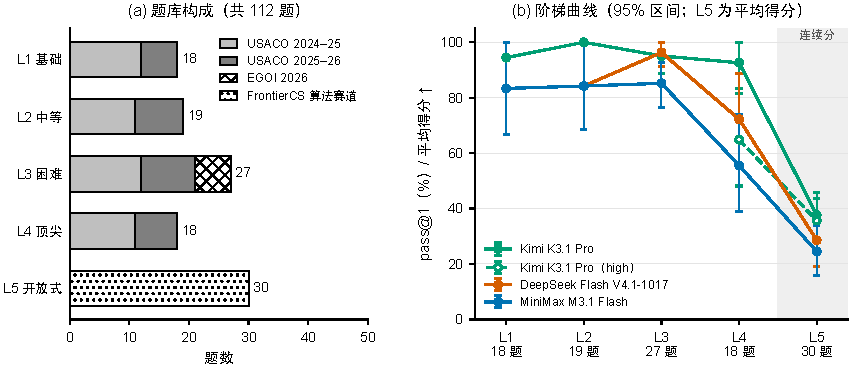
\includegraphics[width=\linewidth]{figures/fig1_overview.pdf}
  \caption{\textbf{codingBench 阶梯评测概览。}(a) 各档题数与来源，图案区分来源。(b) 各模型在各档的主要指标与按题重抽样的 95\% 区间：L1--L4 为 pass@1，L5 为平均得分（连续分）。\kimi 在 L4 与 L5 上分别给出 max（实线）与 high（虚线）两档思考强度的结果。模型之间的差距从 L4 开始明显拉开。}
  \label{fig:overview}
\end{figure}

\section{相关工作}

\paragraph{正确性评测。}HumanEval~\cite{humaneval} 以函数级题目与 pass@$k$ 评测代码生成；APPS~\cite{apps} 与 AlphaCode 的 CodeContests~\cite{alphacode} 把评测扩展到竞赛题。为避免训练数据污染，LiveCodeBench~\cite{lcb} 持续收集新发布的竞赛题；USACO-Bench~\cite{usacobench} 使用 USACO 的历年题目，并按组别报告成绩。CodeElo~\cite{codeelo} 在 Codeforces 上提交并给出与人类可比的 Elo 分，LiveCodeBench Pro~\cite{lcbpro} 由奥赛奖牌得主标注题目难度与类型，OJBench~\cite{ojbench} 收集了 NOI、ICPC 等竞赛级题目。FrontierCS~\cite{frontiercs} 收集没有已知最优解的开放问题，按 checker 给出连续分。与这些工作相比，本文的题库只用官方的测试数据与参考解，并按人类组别分档，便于同时观察各难度段的差距。

\paragraph{效率与质量评测。}EffiBench~\cite{effibench} 与 ENAMEL~\cite{enamel} 比较生成代码与参考解的运行时间，Le 等人~\cite{perfbench} 讨论了性能评测本身的测量问题；BigO(Bench)~\cite{bigobench} 通过规模扫描估计生成代码的时间与空间复杂度；AlgoTune~\cite{algotune} 评测模型能否加速数值程序。Huang 等人~\cite{staticquality} 用 Pylint 与 Radon 等工具分析生成代码的静态质量，本文沿用其工具与版本。SWE-bench~\cite{swebench} 等仓库级、多轮的智能体编程评测考查的是另一种能力，不在本文范围之内。

\paragraph{统计方法。}我们以题目为重抽样单位，用 bootstrap~\cite{efron1979} 估计各档指标与两两差值的区间。

\section{阶梯基准}
\label{sec:bench}

\subsection{设计原则}

\begin{itemize}[leftmargin=1.6em]
  \item \lead{难度用人类标尺划分。}USACO 的四个组别由真实选手的晋级线划定，EGOI 是国际奥赛；档位反映的是人类选手的水平，而不是某个模型觉得难不难。
  \item \lead{只用官方数据。}AtCoder 自 2024 年 12 月起不再公开测试数据，LeetCode 的测试不公开且用户协议禁止批量抓取，这两个来源都给不出可信的标准答案，因此没有采用。
  \item \lead{高档用连续分。}USACO 按测试点给部分分，EGOI 按子任务给分，FrontierCS 由 checker 给出连续分，高档不会像通过率那样很快饱和。
  \item \lead{按官方时限判题。}每个测试点按实际 CPU 时间判定是否在官方时限内完成，与人类选手的判题条件一致；运行效率与复杂度另与官方解比较。
  \item \lead{先验证判题本身。}建库时先用我们的判题程序运行官方题解；没有任何一份官方解能全部通过的题直接剔除，这同时检验了测试数据、比对规则与判题程序。
\end{itemize}

\begin{table}[t]
  \centering
  \caption{\textbf{题库组成。}题数为进入评测的题数。USACO 每个组别计划 21 题，建库校验时剔除了没有官方解能通过、有多个合法答案却没有 checker 等无法可靠判分的题。}
  \label{tab:composition}
  \small
  \begin{tabular}{@{}lllrlll@{}}
    \toprule
    档位 & 来源 & 子集 & 题数 & 比赛时间 & 作答语言 & 计分 \\
    \midrule
    L1 基础 & USACO 铜组 & USACO & 18 & 2024-12 至 2026-02 & Python & 测试点等分 \\
    L2 中等 & USACO 银组 & USACO & 19 & 2024-12 至 2026-02 & Python & 测试点等分 \\
    \multirow{2}{*}{L3 困难} & USACO 金组 & USACO & 21 & 2024-12 至 2026-02 & C++ & 测试点等分 \\
     & EGOI 2026 & 2026 & 6 & 2026-05 & C++ & 子任务取最低分 \\
    L4 顶尖 & USACO 铂金组 & USACO & 18 & 2024-12 至 2026-02 & C++ & 测试点等分 \\
    L5 开放式 & FrontierCS 算法赛道 & FrontierCS & 30 & 题库 v1.1 & C++17 & 0--100 连续分 \\
    \bottomrule
  \end{tabular}
\end{table}

\subsection{题库组成}

表~\ref{tab:composition} 给出了题库组成，共 112 题。USACO~\cite{usaco} 取 2024--25 赛季的 12 月、1 月、2 月与美国公开赛共 4 场，以及 2025--26 赛季的 3 场线上赛（3 月的公开赛为线下监考赛，官网没有公布题目与测试数据）。EGOI 2026~\cite{egoi} 共 8 题，其中 Census 与 Seating Plan 为交互题，不在本题库中。IOI 2026 的题目为通信题或只提供 PDF 题面，未纳入。FrontierCS~\cite{frontiercs,frontiercsrepo} 的题库有 180 道开放式难题，没有类别标签，我们按题号均匀抽取 30 题。题面与测试数据只存放在评测服务器上，不进入代码仓库；仓库只记录题号、档位、日期与时限。

\subsection{构建流程}

构建与评测流程如图~\ref{fig:pipeline} 所示。建库时，每道题的所有官方题解都要在全部测试点上判一遍：没有官方解能全部通过的题被剔除；能通过的官方解中最快的一份作为该题的性能对照。

\begin{figure}[t]
  \centering
  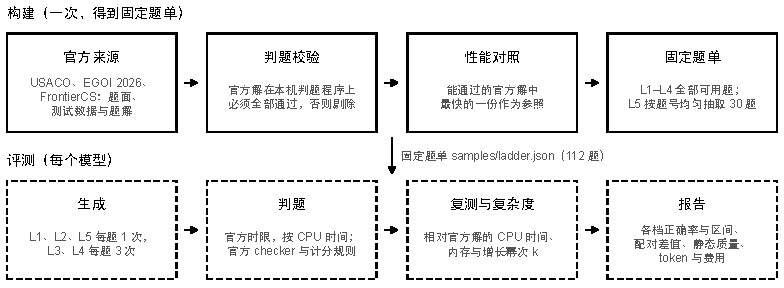
\includegraphics[width=\linewidth]{figures/fig2_pipeline.pdf}
  \caption{\textbf{构建与评测流程。}上行（实线框）只执行一次，得到固定题单；下行（虚线框）对每个模型执行，题目、判题程序与计分规则对所有模型完全相同。}
  \label{fig:pipeline}
\end{figure}

\section{判题、计分与统计方法}

\subsection{运行环境与判定}

判题在评测服务器本机进行。答案以无特权用户运行，由一个小的启动器设置地址空间（内存上限加 64\,MB）、栈、CPU 时间与输出大小（256\,MB）上限，并把进程绑定在一个独占的核上；CPU 时间与峰值内存取自子进程自身的资源统计。CPU 时间超过官方时限的测试点判为超时。Python 档使用 CPython 3.11、只允许标准库，官方时限沿用 USACO 给 Python 的时限；C++ 档以 \texttt{g++ -O2 -std=gnu++17} 编译。USACO 忽略空白逐个 token 比对，与其官方规则一致；EGOI 使用官方 checker；FrontierCS 使用官方的 testlib checker 或交互器，并照搬其判分规则，只解析 checker 输出的得分比例。

\subsection{计分}

每个测试点 $t$ 得分 $s_t \in [0, 1]$：编译失败、运行出错、超时或超内存记 0。每题得分 $S$（0--100）按来源的官方规则计算：USACO 为 $S = 100 \cdot \frac{1}{T}\sum_t s_t$；EGOI 为 $S = 100 \cdot \sum_g w_g \min_{t\in g} s_t / \sum_g w_g$，即子任务 $g$ 取其中测试点的最低分再乘以子任务分值；FrontierCS 为所有测试点得分比例的平均乘以 100，达到参考解为 60 分，超过参考解越多得分越高。所有测试点都满分才算“解出”。L1、L2、L5 每题采样 1 次，L3、L4 每题采样 3 次，以减小高档题少带来的随机误差。pass@1 是解出的采样占全部采样的比例，平均得分是全部采样的 $S$ 的平均，pass@3 是 3 次采样中至少一次解出的题所占比例。L5 为连续分，只报告平均得分。

\subsection{运行效率与复杂度}

只对解出的答案、且官方解在某个测试点上至少需要 0.05 秒 CPU 的题比较运行时间：取官方解最慢的 3 个测试点，答案与官方解交替各运行 3 次取中位数，倍数为答案的 CPU 时间除以官方解的 CPU 时间，各档取几何平均。峰值内存倍数同理。

复杂度方面，官方测试点未按规模排列，USACO 中耗时可测的测试点几乎都是最大规模，直接按输入大小拟合不可行。因此我们以官方解自身的耗时作为规模的度量：在官方解至少需要 2\,ms CPU 的测试点上（最多 20 个，均匀覆盖其耗时范围），答案与官方解交替各运行 5 次取中位数，拟合 $\log y_{\text{答案}} = a + k \log y_{\text{官方}}$。若官方解为 $\Theta(f(n))$、答案为 $\Theta(f(n)^k)$，$k$ 即为这个指数。只在拟合优度 $R^2 \ge 0.8$ 时下结论：$k \le 0.75$ 且在官方解最重的 3 个测试点上答案至少快 2 倍为更优，$0.75 < k < 1.33$ 为同阶，$k \ge 1.33$ 且至少慢 2 倍为更差，其余为不确定；可用测试点少于 4 个或官方耗时跨度不足 4 倍为不可测。

\subsection{静态代码质量}

对 L1、L2 中解出的 Python 答案，按 Huang 等人~\cite{staticquality} 的工具与版本，报告 Pylint 3.3.5 的问题数与 0--10 分，以及 Radon 6.0.1 的圈复杂度、可维护性指数（MI）与代码行数（SLOC）。

\subsection{用量、速度与费用}

每个采样对应一次调用。输出 token 为接口计费的输出用量，含思考过程；延迟为调用从发出到接收完毕的时间；首个 token 时间为从发出到收到第一个 token 的时间；输出速度为输出 token 除以首个 token 之后的时长，单位 tokens/s。各档报告每次调用的平均输出 token 与输出速度、首个 token 时间、延迟的中位数。费用按各家的官方美元标价计算：$(\text{输入} - \text{缓存命中}) \times \text{输入单价} + \text{缓存命中} \times \text{命中单价} + \text{输出} \times \text{输出单价}$，分时计价按每次调用的开始时间。

\subsection{统计方法}

模型之间的比较以题目为单位。各档指标的 95\% 区间来自 $B = 2000$ 次按题重抽样（随机种子 0）：每次在每档内部有放回地抽取同样数量的题，重新计算各档与 L1--L4 合计的 pass@1 与平均得分，取 2.5\% 与 97.5\% 分位数；两个模型使用同一组题（配对 bootstrap），从而消除题目难度带来的共同波动。逐题比较取每题所有采样的平均得分，相差不到 0.05 分记为持平，并对胜负题数做精确符号检验。

\section{实验设置}

\subsection{被测模型}

三个模型都在 2026 年 9--10 月发布，都默认开启思考。下面依次概述它们的能力、厂商公开的技术要点及其所针对的能力，以及官方的代码评测成绩。以下内容来自厂商的技术博客、技术报告、模型卡与接口文档，分数为厂商自报。

\paragraph{\kimi。}月之暗面于 2026 年 10 月 23 日发布，官方称它是 Kimi K3 的后训练版本，使用了大得多的后训练算力，并在数百个下游领域上联合做强化学习~\cite{kimik31}；K3 为 MoE 架构，总参数 2.8T、每 token 激活 104B，上下文 1M~\cite{kimik3}。代码方面，官方称 K3.1 Pro 覆盖从真实代码库中的快速修复到完整项目构建的全部编程工作，并以大规模强化学习增强长程编程；自报 Terminal-Bench 4.0 65.7\%（Claude Code 框架），内部的 Kimi Code Bench 3.0 长程子集 61.2\%（K3 为 55.95\%）。官方成绩使用 max 思考强度、temperature 1.0、top-p 0.95；另有 Highspeed 版本（\texttt{kimi-k3.1-pro-highspeed}），称速度为 K3.1 Pro 的 2--3 倍~\cite{kimik31}。思考不能关闭，强度可选 low、high、max，不指定时默认 max~\cite{kimieffort}。官方没有报告竞赛编程成绩。

\paragraph{\ds。}DeepSeek 于 2026 年 9 月 10 日发布 V4.1-Flash，10 月 17 日更新为 1017 版，接口名与价格不变，以 MIT 许可开放权重~\cite{ds1017}。模型为多模态 MoE，主干 552B 参数、每 token 激活 8B（prefill）/ 16B（decode），另有 196B 的 Engram 条件记忆，上下文 1M。技术报告~\cite{dsv41} 的主要创新在注意力与 KV cache 的压缩，面向长上下文与“输入很重”的智能体场景的服务成本；报告明确说后训练“没有算法上的创新”，沿用监督微调、强化学习与在线蒸馏的标准流程，改动都在数据上，并在训练中按思考深度施加长度惩罚，使深度可调。报告称其 Codeforces 评分（内部评测）为 3471，高于 V4-Flash 的 3289 与 V4-Pro 的 3348。1017 版称以自反馈强化学习改进端到端的项目开发，并缩短了任务耗时与输出长度；厂商自报（智能体框架）Terminal-Bench 4.0 由 31.2 提高到 42.3、DeepSWE v1.1 由 74.2 提高到 77.0、ProgramBench 由 20.3 提高到 29.1~\cite{ds1017}。官方评测使用最高思考深度，接口不指定时默认为 high~\cite{dsapi}。

\paragraph{\mini。}MiniMax 于 2026 年 10 月 19 日上线接口、10 月 23 日开放权重；MoE 架构，总参数约 428B、每 token 激活约 23B，上下文 1M，思考不能关闭，不指定时默认最高深度~\cite{minimaxm31}。厂商称 M3.1 Flash 沿用前代 M3 的核心架构，只做了三处改动：全部层改为稀疏注意力，路由专家与注意力路径做量化感知训练，以 DSpark 投机解码代替原先的多 token 预测。这三处都面向推理速度与成本：官方称输出速度可达每秒 200 token 以上、中位数稳定在 170 以上，在线推理快近 3 倍、使用成本降低 70\%。厂商把它定位于智能体任务，称其原生支持在每轮工具调用之间思考（交错思考），自报 DeepSWE v1.1 73.7、Terminal Bench 4.0 38.1、NL2Repo-Bench 61.2~\cite{minimaxm31}；前代 M3 自报 SWE-Bench Verified 80.5~\cite{minimaxm3}。

三家都没有报告与本文题源重合的评测（USACO、EGOI 或 FrontierCS）：\ds 的技术报告只在思考深度的曲线图中给出 LiveCodeBench（未注明版本、没有数值表），\kimi 与 \mini 没有报告竞赛编程成绩。

\subsection{调用设置}

三个模型都通过各自厂商的官方接口流式调用（表~\ref{tab:models}）。\mini 的 temperature 为 0.2、top\_p 为 0.95（沿用 LiveCodeBench 的设置）；\ds 在思考模式下不支持 temperature 参数~\cite{dsapi}；\kimi 不传 temperature 与 top\_p，使用接口默认值。

\paragraph{思考强度。}三家接口都提供思考强度参数（\texttt{reasoning\_effort}）。本文把请求中不指定思考强度、由接口采用默认值的设置记为 auto：\kimi 与 \mini 的默认值为 max，\ds 的默认值为 high。各模型的思考强度见表~\ref{tab:models}。\kimi 在 L4、L5 上给出 high 与 max 两组结果：high 一组以 high 作答全部 84 个采样；max 一组中，L5 的 30 个采样与 L4 中 high 下输出有误的 18 个采样以 max 作答，L4 其余 36 个采样沿用 high 的答案。

\begin{table}[t]
  \centering
  \caption{\textbf{被测模型与调用设置。}单价为各厂商的公开标价（美元 / 百万 token），依次为输入（缓存未命中）、缓存命中与输出；\ds 在北京时间非高峰时段半价，费用按每次调用的开始时间计算。auto 表示请求中不指定思考强度，括号内为接口默认值。}
  \label{tab:models}
  \small
  \begin{tabularx}{\linewidth}{@{}>{\raggedright\arraybackslash}p{2.6cm}>{\raggedright\arraybackslash}p{2.5cm}>{\raggedright\arraybackslash}X>{\raggedright\arraybackslash}p{1.7cm}>{\raggedright\arraybackslash}p{2.3cm}@{}}
    \toprule
    模型 & API 名称 & 思考强度 & 输出上限 & 单价 \\
    \midrule
    \kimi & kimi-k3.1-pro & L1--L3：auto（max）；L4--L5：max & 262,144；max 为 1,046,528 & 2.00 / 0.20 / 10.00 \\
    \kimi（high） & kimi-k3.1-pro & L4--L5：high & 262,144 & 2.00 / 0.20 / 10.00 \\
    \ds & deepseek-flash & L1--L5：auto（high） & 262,144 & 0.30 / 0.006 / 1.20（非高峰半价） \\
    \mini & MiniMax-M3.1-Flash & L1--L5：auto（max）；L4 中 9 个、L5 中 1 个采样为 high & 262,144 & 0.15 / 0.015 / 0.60 \\
    \bottomrule
  \end{tabularx}
\end{table}

\subsection{归因规则}

厂商声称的改进大多相对其上一代模型而言，而本文没有评测它们的前代，因此不检验“是否比前代更好”，而检验较弱的命题：厂商声称擅长或改进的方向，在本文对应的测量上是否表现为显著的相对优势。一条声称同时满足以下两点时，记为一致，可归因：

\begin{itemize}[leftmargin=1.6em]
  \item 厂商指明了它针对的能力，且能对应到本文的某个档位或某项测量（正确率、运行效率、生成速度、输出长度等）；
  \item 在这项测量上，该模型相对另一个模型的差值显著（区间不含 0），方向与声称一致；对于可直接测量的绝对数值（如生成速度），本文的测量值与声称相符。
\end{itemize}

方向相反或测量值与声称不符时记为不一致；对应不到本文测量的声称（如多轮的智能体编程）记为超出测量范围；只是相对前代的数量声称，记为无法检验；观测到显著差异但没有对应声称的，记为无对应声称，不作归因。三个模型在数据、规模与训练方法上同时不同，本文没有消融实验，这种归因说明观测与声称是否相符，不说明因果。

\section{实验结果}

\subsection{主要结果}

表~\ref{tab:main} 与图~\ref{fig:scores} 给出了各模型在各档的正确率。

\begin{table}[t]
  \centering
  \caption{\textbf{各档正确率。}方括号内为按题重抽样的 95\% 区间；每档最高值加粗。L5 为连续分，只报告平均得分；pass@3 只适用于每题 3 次采样的 L3、L4。}
  \label{tab:main}
  \small
  \begin{adjustbox}{max width=\linewidth}\begin{tabular}{@{}llrrrr@{}}
\toprule
档位 & 模型 & 采样数 & pass@1（\%）$\uparrow$ [95\% 区间] & 平均得分 $\uparrow$ [95\% 区间] & pass@3（\%）$\uparrow$ \\
\midrule
\multirow{3}{*}{L1 基础} & Kimi & 18 & \textbf{94.4} [83.3, 100.0] & \textbf{97.0} [91.0, 100.0] & -- \\
 & DeepSeek & 18 & 83.3 [66.7, 100.0] & 94.7 [87.3, 100.0] & -- \\
 & MiniMax & 18 & 83.3 [66.7, 100.0] & 88.5 [72.9, 100.0] & -- \\
\cmidrule(lr){1-6}
\multirow{3}{*}{L2 中等} & Kimi & 19 & \textbf{100.0} [100.0, 100.0] & \textbf{100.0} [100.0, 100.0] & -- \\
 & DeepSeek & 19 & 84.2 [68.4, 100.0] & 95.2 [89.8, 100.0] & -- \\
 & MiniMax & 19 & 84.2 [68.4, 100.0] & 87.0 [71.6, 100.0] & -- \\
\cmidrule(lr){1-6}
\multirow{3}{*}{L3 困难} & Kimi & 81 & 95.1 [88.9, 100.0] & 96.3 [90.5, 100.0] & 100.0 \\
 & DeepSeek & 81 & \textbf{96.3} [91.4, 100.0] & \textbf{98.3} [95.5, 100.0] & 100.0 \\
 & MiniMax & 81 & 85.2 [76.5, 92.6] & 88.1 [80.8, 94.6] & 100.0 \\
\cmidrule(lr){1-6}
\multirow{4}{*}{L4 顶尖} & Kimi & 54 & \textbf{92.6} [83.3, 100.0] & \textbf{95.4} [88.3, 100.0] & 100.0 \\
 & Kimi（high） & 54 & 64.8 [48.1, 81.5] & 72.9 [58.2, 86.3] & 88.9 \\
 & DeepSeek & 54 & 72.2 [55.6, 88.9] & 76.6 [62.8, 90.0] & 88.9 \\
 & MiniMax & 54 & 55.6 [38.9, 74.1] & 59.1 [43.4, 75.7] & 77.8 \\
\cmidrule(lr){1-6}
\multirow{4}{*}{L5 开放式} & Kimi & 30 & -- & \textbf{37.6} [28.6, 45.9] & -- \\
 & Kimi（high） & 30 & -- & 35.7 [27.9, 43.8] & -- \\
 & DeepSeek & 30 & -- & 28.6 [19.0, 38.2] & -- \\
 & MiniMax & 30 & -- & 24.5 [15.9, 33.9] & -- \\
\cmidrule(lr){1-6}
\multirow{3}{*}{L1--L4 合计} & Kimi & 172 & \textbf{94.8} [90.7, 98.3] & \textbf{96.5} & -- \\
 & DeepSeek & 172 & 86.0 [79.7, 91.9] & 90.7 & -- \\
 & MiniMax & 172 & 75.6 [69.2, 83.1] & 78.9 & -- \\
\bottomrule
\end{tabular}
\end{adjustbox}
\end{table}

\begin{figure}[t]
  \centering
  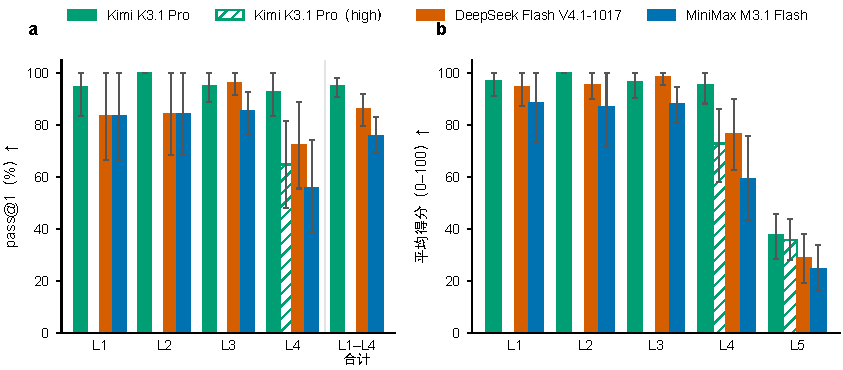
\includegraphics[width=\linewidth]{figures/fig3_scores.pdf}
  \caption{\textbf{各档正确率与 95\% 区间。}(a) pass@1，最右为 L1--L4 合计；(b) 平均得分。斜线柱为 \kimi 在 high 思考强度下的结果。}
  \label{fig:scores}
\end{figure}

\lead{\kimi 的 L1--L4 合计 pass@1 最高，差距集中在 L4。}L1--L4 合计，\kimi 的 pass@1 为 94.8\%（区间 90.7 至 98.3），\ds 为 86.0\%（79.7 至 91.9），\mini 为 75.6\%（69.2 至 83.1）。L4 上三者分别为 92.6\%、72.2\% 与 55.6\%，\kimi 领先 \ds{} 20.4 个百分点、领先 \mini{} 37.0 个百分点。L3 上 \kimi 与 \ds 分别为 95.1\% 与 96.3\%，3 次采样中至少解出一次的比例三者都是 100\%。

\lead{\ds{} 在 L1、L2 的失分全部来自官方时限。}L1、L2 上 \kimi 的 pass@1 为 94.4\% 与 100\%，\ds 与 \mini 均为 83.3\% 与 84.2\%。\ds 在这两档没有解出的 6 个采样全部是输出正确、但 CPU 时间超过官方时限的 Python 答案（表~\ref{tab:fail}）。

\lead{L5 三个模型都远低于参考解。}L5 的平均得分分别为 37.6（\kimi）、28.6（\ds）与 24.5（\mini），官方参考解为 60 分；没有一个答案在全部测试点上取得满分。

\subsection{模型之间的差距是否可信？}

表~\ref{tab:pairwise} 与图~\ref{fig:pairwise} 给出了三组两两比较的配对差值与逐题胜负。

\begin{table}[t]
  \centering
  \caption{\textbf{两两比较。}L1--L4 与合计为 pass@1 之差（百分点），L5 为平均得分之差；方括号内为配对 bootstrap 的 95\% 区间，$^{*}$ 表示区间不含 0。胜/平/负为逐题比较的题数（以每题所有采样的平均得分比较）。}
  \label{tab:pairwise}
  \small
  \begin{adjustbox}{max width=\linewidth}\begin{tabular}{@{}lrrrrrr@{}}
\toprule
 & \multicolumn{2}{c}{Kimi $-$ DeepSeek} & \multicolumn{2}{c}{Kimi $-$ MiniMax} & \multicolumn{2}{c}{DeepSeek $-$ MiniMax} \\
\cmidrule(lr){2-3}\cmidrule(lr){4-5}\cmidrule(lr){6-7}
档位 & 差值 [95\% 区间] & 胜/平/负 & 差值 [95\% 区间] & 胜/平/负 & 差值 [95\% 区间] & 胜/平/负 \\
\midrule
L1 基础 & +11.1 [0.0, 27.8] & 2/16/0 & +11.1 [0.0, 27.8] & 2/15/1 & +0.0 [$-$22.2, 22.2] & 2/13/3 \\
L2 中等 & +15.8 [0.0, 31.6] & 3/16/0 & +15.8 [0.0, 31.6] & 3/16/0 & +0.0 [$-$15.8, 15.8] & 3/15/1 \\
L3 困难 & $-$1.2 [$-$8.6, 4.9] & 3/21/3 & +9.9$^{*}$ [1.2, 18.5] & 9/16/2 & +11.1$^{*}$ [3.7, 19.8] & 9/16/2 \\
L4 顶尖 & +20.4$^{*}$ [5.6, 37.0] & 8/9/1 & +37.0$^{*}$ [18.5, 55.6] & 12/5/1 & +16.7$^{*}$ [5.6, 29.6] & 11/6/1 \\
\midrule
L1--L4 合计 & +8.7$^{*}$ [2.3, 15.1] & -- & +19.2$^{*}$ [11.6, 26.7] & -- & +10.5$^{*}$ [4.7, 16.9] & -- \\
\midrule
L5 开放式 & +9.0$^{*}$ [0.6, 17.7] & 15/7/8 & +13.1$^{*}$ [3.4, 22.6] & 17/7/6 & +4.1 [$-$4.3, 12.5] & 14/7/9 \\
\midrule
全部 112 题（逐题符号检验） &  & 31/69/12，$p=0.005$ &  & 43/59/10，$p<0.001$ &  & 39/57/16，$p=0.003$ \\
\bottomrule
\end{tabular}
\end{adjustbox}
\end{table}

\begin{figure}[t]
  \centering
  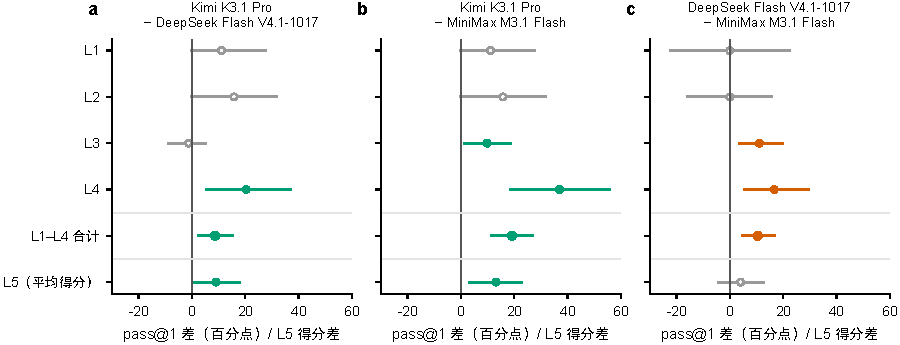
\includegraphics[width=\linewidth]{figures/fig4_pairwise.pdf}
  \caption{\textbf{两两比较的差值与 95\% 区间。}实心点为区间不含 0 的差值，颜色为领先的一方；空心灰点为区间含 0。}
  \label{fig:pairwise}
\end{figure}

\lead{三组差距在 L1--L4 合计上都显著。}\kimi 领先 \ds{} 8.7 个百分点（区间 2.3 至 15.1），领先 \mini{} 19.2 个百分点（11.6 至 26.7）；\ds 领先 \mini{} 10.5 个百分点（4.7 至 16.9）。逐题比较全部 112 题，\kimi 对 \ds 为 31 胜 12 负（$p = 0.005$），对 \mini 为 43 胜 10 负（$p < 0.001$），\ds 对 \mini 为 39 胜 16 负（$p = 0.003$）。

\lead{显著差距出现在 L3 以上。}L1、L2 的差值区间都含 0。\kimi 与 \ds 在 L3 上没有差别（$-1.2$，区间 $-8.6$ 至 4.9），在 L4 与 L5 上 \kimi 显著领先（$+20.4$ 与 $+9.0$）。\ds 与 \mini 的差距在 L3、L4 上显著（$+11.1$ 与 $+16.7$），在 L5 上不显著（$+4.1$，区间 $-4.3$ 至 12.5）。

\subsection{思考强度的影响}

表~\ref{tab:effort}、表~\ref{tab:effortcost} 与图~\ref{fig:effort} 比较了 \kimi 在 L4、L5 上的 high 与 max 两档思考强度。

\begin{table}[t]
  \centering
  \caption{\textbf{\kimi 的 high 与 max。}L4 为 high 下输出有误的 18 个采样，L5 为全部 30 个采样；差值为 max 减 high 的平均得分，方括号内为按采样重抽样的 95\% 区间；提高/持平/降低按得分变化是否达到 0.05 分计，$p$ 为精确符号检验。}
  \label{tab:effort}
  \small
  \begin{adjustbox}{max width=\linewidth}\begin{tabular}{@{}lrrrrr@{}}
\toprule
比较范围 & 采样数 & 解出 high $\rightarrow$ max & 平均得分 high $\rightarrow$ max & 差值 [95\% 区间] & 提高/持平/降低 \\
\midrule
L4（high 未解出的采样） & 18 & 0 $\rightarrow$ 15 & 19.4 $\rightarrow$ 86.9 & +67.6 [48.4, 84.7] & 15/2/1，$p<0.001$ \\
L5（全部采样） & 30 & -- & 35.7 $\rightarrow$ 37.6 & +2.0 [$-$6.0, 10.4] & 8/10/12，$p=0.50$ \\
\bottomrule
\end{tabular}
\end{adjustbox}
\end{table}

\begin{table}[t]
  \centering
  \caption{\textbf{high 与 max 的输出长度、速度与延迟}（与表~\ref{tab:effort} 为同一批采样）。输出 token 含思考；速度与延迟为中位数。}
  \label{tab:effortcost}
  \small
  \begin{tabular}{@{}llrrr@{}}
\toprule
档位 & 思考强度 & 每次输出 token $\downarrow$ & 输出速度（tokens/s）$\uparrow$ & 延迟中位数（分钟）$\downarrow$ \\
\midrule
\multirow{2}{*}{L4 顶尖} & high & 43.8k & 23.3 & 27.6 \\
 & max & 71.6k & 24.6 & 41.3 \\
\cmidrule(lr){1-5}
\multirow{2}{*}{L5 开放式} & high & 15.3k & 25.4 & 9.2 \\
 & max & 34.4k & 28.4 & 20.2 \\
\bottomrule
\end{tabular}

\end{table}

\begin{figure}[t]
  \centering
  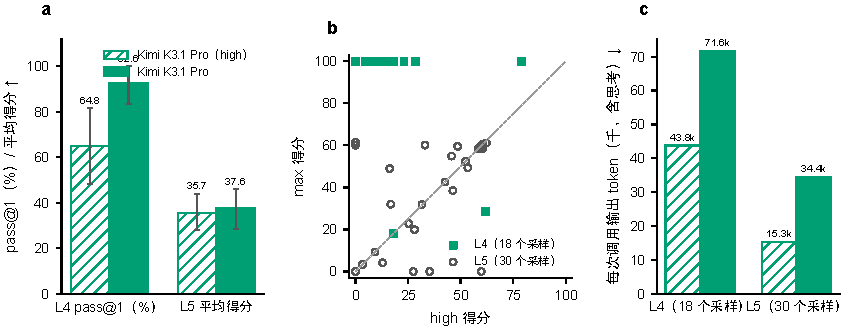
\includegraphics[width=\linewidth]{figures/fig5_effort.pdf}
  \caption{\textbf{\kimi 的 high 与 max。}(a) L4 的 pass@1 与 L5 的平均得分，误差线为 95\% 区间；(b) 逐个采样的得分，方块为 L4 中 high 下输出有误的 18 个采样，圆圈为 L5 的 30 个采样，虚线为两档相等；(c) 同一批采样每次调用的平均输出 token。}
  \label{fig:effort}
\end{figure}

\lead{max 显著提高了 L4，对 L5 没有显著影响。}L4 的 pass@1 由 high 的 64.8\% 升至 max 的 92.6\%，差 27.8 个百分点（区间 14.8 至 42.6），逐题比较 10 题提高、无一降低（$p = 0.002$）。在 high 下输出有误的 18 个采样中，max 解出 15 个，平均得分由 19.4 升至 86.9。L5 的平均得分由 35.7 升至 37.6，差 2.0 分（区间 $-$6.0 至 10.4），30 题中 8 题提高、12 题降低（$p = 0.50$）；其中 fcs-85 与 fcs-104 的 max 答案编译失败，high 答案能够编译。

\lead{max 的输出更长，速度不变。}在同一批采样上，max 每次调用的平均输出 token 在 L4 为 high 的 1.6 倍（71.6k 对 43.8k），在 L5 为 2.2 倍（34.4k 对 15.3k）；两档的输出速度都在每秒 23 至 29 token 之间，延迟随输出长度同步增加。

\lead{思考强度改变了 L4 的排名。}L4 上 high 的 64.8\% 介于 \ds（72.2\%）与 \mini（55.6\%）之间，max 的 92.6\% 则高于两者；L5 上 high 的 35.7 分已高于 \ds 的 28.6 与 \mini 的 24.5。

\subsection{新题是否明显更难？}

表~\ref{tab:subsets} 把 L3、L4 分为 EGOI 2026 新题与 USACO 两个赛季。

\begin{table}[t]
  \centering
  \caption{\textbf{新旧题对照（pass@1，\%）。}EGOI 2026 发布于 2026 年 5 月，晚于 USACO 的全部比赛。}
  \label{tab:subsets}
  \small
  \begin{tabular}{@{}llrrrrr@{}}
\toprule
档位 & 子集 & 题数 & Kimi & Kimi（high） & DeepSeek & MiniMax \\
\midrule
\multirow{3}{*}{L3 困难} & EGOI 2026 & 6 & 100.0 & -- & 100.0 & 83.3 \\
 & USACO 2024--25 & 12 & 100.0 & -- & 94.4 & 86.1 \\
 & USACO 2025--26 & 9 & 85.2 & -- & 96.3 & 85.2 \\
\cmidrule(lr){1-7}
\multirow{2}{*}{L4 顶尖} & USACO 2024--25 & 11 & 100.0 & 81.8 & 75.8 & 66.7 \\
 & USACO 2025--26 & 7 & 81.0 & 38.1 & 66.7 & 38.1 \\
\bottomrule
\end{tabular}

\end{table}

\lead{最新的 EGOI 2026 题没有比旧题更差。}\kimi 与 \ds 解出了 EGOI 2026 的全部 18 个采样，\mini 为 83.3\%，与其 L3 的 USACO 2024--25 子集（86.1\%）相当。三个模型在最新题上都没有表现出系统性下降，这一对照没有显示训练数据泄露的迹象。

\lead{L4 上 USACO 2025--26 赛季的题对三个模型都更难。}\kimi 在 2024--25 赛季解出全部 33 个采样，在 2025--26 赛季为 81.0\%；\ds 由 75.8\% 降至 66.7\%，\mini 由 66.7\% 降至 38.1\%。L3 上只有 \kimi 出现同样的下降（100\% 降至 85.2\%），\ds 与 \mini 在两个赛季之间相差不到 2 个百分点。

\subsection{解出的答案有多快？}

表~\ref{tab:perf} 与表~\ref{tab:cplx} 给出了解出答案相对官方解的运行效率与复杂度。

\begin{table}[t]
  \centering
  \caption{\textbf{运行效率（相对官方解，同语言）。}只比较解出的答案；倍数为各档的几何平均，小于 1 表示快于官方解。EGOI 与 FrontierCS 没有官方解，不参与比较。}
  \label{tab:perf}
  \small
  \begin{tabular}{@{}llrrrrr@{}}
\toprule
档位 & 模型 & 比较的答案数 & CPU 时间倍数 $\downarrow$ & 快于官方解 & 慢 2 倍以上 & 峰值内存倍数 $\downarrow$ \\
\midrule
\multirow{3}{*}{L1 基础} & Kimi & 12 & 0.47$\times$ & 10 & 2 & 0.95$\times$ \\
 & DeepSeek & 11 & 0.49$\times$ & 10 & 1 & 0.98$\times$ \\
 & MiniMax & 10 & 0.42$\times$ & 9 & 1 & 0.80$\times$ \\
\cmidrule(lr){1-7}
\multirow{3}{*}{L2 中等} & Kimi & 9 & 0.87$\times$ & 6 & 0 & 1.25$\times$ \\
 & DeepSeek & 8 & 0.81$\times$ & 7 & 0 & 1.34$\times$ \\
 & MiniMax & 8 & 0.54$\times$ & 8 & 0 & 1.14$\times$ \\
\cmidrule(lr){1-7}
\multirow{3}{*}{L3 困难} & Kimi & 56 & 0.63$\times$ & 43 & 0 & 0.90$\times$ \\
 & DeepSeek & 57 & 0.56$\times$ & 47 & 2 & 0.89$\times$ \\
 & MiniMax & 51 & 0.45$\times$ & 43 & 0 & 0.83$\times$ \\
\cmidrule(lr){1-7}
\multirow{4}{*}{L4 顶尖} & Kimi & 47 & 0.75$\times$ & 33 & 4 & 1.11$\times$ \\
 & Kimi（high） & 32 & 0.74$\times$ & 23 & 3 & 1.11$\times$ \\
 & DeepSeek & 36 & 0.94$\times$ & 18 & 8 & 1.26$\times$ \\
 & MiniMax & 27 & 0.54$\times$ & 22 & 2 & 0.98$\times$ \\
\bottomrule
\end{tabular}

\end{table}

\begin{table}[t]
  \centering
  \caption{\textbf{时间复杂度（相对官方解，答案数）。}按第 4.3 节的增长幂次 $k$ 分类；$k$ 中位数只统计更优、同阶与更差三类。}
  \label{tab:cplx}
  \small
  \begin{tabular}{@{}llrrrrrr@{}}
\toprule
档位 & 模型 & 更优 & 同阶 & 更差 & 不确定 & 不可测 & $k$ 中位数 \\
\midrule
\multirow{3}{*}{L1 基础} & Kimi & 1 & 7 & 0 & 3 & 1 & 0.85 \\
 & DeepSeek & 1 & 4 & 0 & 2 & 4 & 0.91 \\
 & MiniMax & 4 & 4 & 0 & 2 & 0 & 0.74 \\
\cmidrule(lr){1-8}
\multirow{3}{*}{L2 中等} & Kimi & 0 & 8 & 0 & 0 & 1 & 0.97 \\
 & DeepSeek & 0 & 5 & 0 & 0 & 3 & 1.01 \\
 & MiniMax & 1 & 6 & 0 & 1 & 0 & 0.87 \\
\cmidrule(lr){1-8}
\multirow{3}{*}{L3 困难} & Kimi & 7 & 42 & 0 & 10 & 0 & 0.98 \\
 & DeepSeek & 4 & 42 & 1 & 10 & 3 & 0.96 \\
 & MiniMax & 16 & 29 & 0 & 9 & 0 & 0.92 \\
\cmidrule(lr){1-8}
\multirow{4}{*}{L4 顶尖} & Kimi & 4 & 37 & 2 & 4 & 0 & 0.95 \\
 & Kimi（high） & 2 & 26 & 1 & 3 & 0 & 0.95 \\
 & DeepSeek & 4 & 27 & 0 & 1 & 4 & 0.95 \\
 & MiniMax & 6 & 20 & 0 & 1 & 0 & 0.90 \\
\bottomrule
\end{tabular}

\end{table}

\lead{三个模型解出的答案普遍快于官方解。}各档 CPU 时间倍数的几何平均都在 0.42 至 0.94 之间。L4 上 \mini 的倍数最低（0.54），\kimi 为 0.75，\ds 为 0.94；\ds 在 L4 有 8 份答案慢于官方解 2 倍以上，\kimi 为 4 份，\mini 为 2 份。三个模型解出的题并不相同，\mini 解出的 L4 题最少，这一比较只针对各自解出的答案。

\lead{复杂度与官方解同阶的答案占多数。}L3、L4 中可判定的答案大多与官方解同阶；判为更差的答案共 3 份（\kimi 在 L4 有 2 份，\ds 在 L3 有 1 份）。\mini 在 L3 有 16 份答案的增长慢于官方解，\kimi 与 \ds 分别为 7 份与 4 份。

\subsection{答案为什么没有解出？}

表~\ref{tab:fail} 按第一个成立的原因对未解出的答案分类。

\begin{table}[t]
  \centering
  \caption{\textbf{失败类型（答案数）。}每份答案只记一个主要原因，判定顺序为无代码、生成超时、编译错误、答案错误、运行错误、超时、部分分；生成超时指接口在返回答案前断开；L5 为连续计分，得分大于 0 的答案记为部分分。}
  \label{tab:fail}
  \small
  \begin{adjustbox}{max width=\linewidth}\begin{tabular}{@{}llrrrrrrrrr@{}}
\toprule
档位 & 模型 & 答案数 & 未解出 & 无代码 & 生成超时 & 编译错误 & 答案错误 & 运行错误 & 超时 & 部分分 \\
\midrule
\multirow{3}{*}{L1 基础} & Kimi & 18 & 1 & 0 & 0 & 0 & 0 & 0 & 1 & 0 \\
 & DeepSeek & 18 & 3 & 0 & 0 & 0 & 0 & 0 & 3 & 0 \\
 & MiniMax & 18 & 3 & 0 & 0 & 0 & 1 & 1 & 1 & 0 \\
\cmidrule(lr){1-10}
\multirow{3}{*}{L2 中等} & Kimi & 19 & 0 & 0 & 0 & 0 & 0 & 0 & 0 & 0 \\
 & DeepSeek & 19 & 3 & 0 & 0 & 0 & 0 & 0 & 3 & 0 \\
 & MiniMax & 19 & 3 & 0 & 0 & 0 & 2 & 0 & 1 & 0 \\
\cmidrule(lr){1-10}
\multirow{3}{*}{L3 困难} & Kimi & 81 & 4 & 0 & 0 & 0 & 4 & 0 & 0 & 0 \\
 & DeepSeek & 81 & 3 & 0 & 0 & 0 & 2 & 0 & 1 & 0 \\
 & MiniMax & 81 & 12 & 0 & 0 & 3 & 9 & 0 & 0 & 0 \\
\cmidrule(lr){1-10}
\multirow{4}{*}{L4 顶尖} & Kimi & 54 & 4 & 0 & 0 & 0 & 3 & 0 & 1 & 0 \\
 & Kimi（high） & 54 & 19 & 0 & 0 & 0 & 18 & 0 & 1 & 0 \\
 & DeepSeek & 54 & 15 & 1 & 0 & 0 & 12 & 1 & 1 & 0 \\
 & MiniMax & 54 & 24 & 0 & 1 & 11 & 12 & 0 & 0 & 0 \\
\cmidrule(lr){1-10}
\multirow{4}{*}{L5 开放式} & Kimi & 30 & 30 & 0 & 0 & 2 & 2 & 1 & 0 & 25 \\
 & Kimi（high） & 30 & 30 & 0 & 0 & 1 & 2 & 0 & 0 & 27 \\
 & DeepSeek & 30 & 30 & 2 & 0 & 1 & 4 & 0 & 0 & 23 \\
 & MiniMax & 30 & 30 & 0 & 0 & 7 & 4 & 0 & 2 & 17 \\
\bottomrule
\end{tabular}
\end{adjustbox}
\end{table}

\lead{答案错误是 L3、L4 的主要原因，\mini 另有大量编译错误。}L4 上，\kimi 未解出的 4 个采样中 3 个为答案错误、1 个为超时；\ds 的 15 个中 12 个为答案错误；\mini 的 24 个中 12 个为答案错误、11 个为编译错误。L5 上 \mini 有 7 份答案编译失败，\kimi 与 \ds 分别为 2 份与 1 份。

\lead{低档的失败以超时为主。}L1、L2 上 \ds 的 6 个未解出采样都是超时，\kimi 只有 1 个；\mini 的 6 个中 3 个为答案错误、2 个为超时、1 个为运行错误。

\subsection{代码质量}

表~\ref{tab:quality} 给出了 L1、L2 中解出的 Python 答案的静态质量。

\begin{table}[t]
  \centering
  \caption{\textbf{静态代码质量（L1、L2 中解出的 Python 答案，每份平均）。}每列较好者加粗，SLOC 不比较优劣。}
  \label{tab:quality}
  \small
  \begin{tabular}{@{}lrrrrrrr@{}}
\toprule
 & & \multicolumn{3}{c}{Pylint 3.3.5} & \multicolumn{3}{c}{Radon 6.0.1} \\
\cmidrule(lr){3-5}\cmidrule(lr){6-8}
模型 & 答案数 & 问题数 $\downarrow$ & 得分 $\uparrow$ & 每百行问题数 $\downarrow$ & 圈复杂度 $\downarrow$ & 可维护性 MI $\uparrow$ & SLOC \\
\midrule
Kimi & 36 & 5.31 & 8.91 & \textbf{9.38} & \textbf{14.67} & 57.7 & 56.6 \\
DeepSeek & 31 & 8.23 & 8.72 & 12.62 & 18.58 & 51.4 & 65.2 \\
MiniMax & 31 & \textbf{5.03} & \textbf{8.96} & 9.47 & 14.87 & \textbf{62.6} & 53.1 \\
\bottomrule
\end{tabular}

\end{table}

\kimi 与 \mini 的质量指标相近：Pylint 问题数分别为 5.31 与 5.03，每百行问题数为 9.38 与 9.47，圈复杂度为 14.67 与 14.87。\ds 的答案更长（SLOC 65.2），问题数（8.23）与圈复杂度（18.58）更高，可维护性指数更低（51.4）。三者的 Pylint 得分都在 8.7 分以上。

\subsection{观测到的差异能否归因于厂商声称的技术改进？}

表~\ref{tab:attr} 按第 5.3 节的规则，把第 5.1 节列出的技术声称与本文的观测逐条对照。

{\small
\begin{longtable}{@{}>{\raggedright\arraybackslash}p{4.0cm}>{\raggedright\arraybackslash}p{1.6cm}>{\raggedright\arraybackslash}p{6.9cm}>{\raggedright\arraybackslash}p{2.2cm}@{}}
  \caption{\textbf{厂商声称与本文观测的对照。}差值为该模型减去对比模型，方括号内为配对 bootstrap 的 95\% 区间。}\label{tab:attr}\\
    \toprule
    厂商声称 & 对应维度 & 本文观测 & 判定 \\
    \midrule
    \endfirsthead
    \toprule
    厂商声称 & 对应维度 & 本文观测 & 判定 \\
    \midrule
    \endhead
    \multicolumn{4}{@{}l}{\textbf{\kimi}} \\
    以大规模强化学习增强长程编程（Kimi Code Bench 3.0 长程 61.2，K3 为 55.95） & 多轮、多文件编程 & 本文为单轮、单文件、无工具的作答 & 超出测量范围 \\
    智能体编程（Terminal-Bench 4.0 65.7） & 多轮、带工具 & 同上 & 超出测量范围 \\
    官方成绩以 max 思考强度取得 & 思考强度 & max 相对 high：L4 pass@1 $+$27.8 [14.8, 42.6]；L5 平均得分 $+$2.0 [$-$6.0, 10.4] & L4 一致；L5 差异不显著 \\
    Highspeed 版本速度为 K3.1 Pro 的 2--3 倍 & 生成速度 & 本文评测的是 kimi-k3.1-pro，输出速度中位数 25.6 tokens/s & 超出测量范围 \\
    没有竞赛编程方面的声称或成绩 & 竞赛编程 & L4 领先 \ds{} $+$20.4 [5.6, 37.0]、领先 \mini{} $+$37.0 [18.5, 55.6]；L5 领先 $+$9.0 与 $+$13.1 & 无对应声称 \\
    \midrule
    \multicolumn{4}{@{}l}{\textbf{\ds}} \\
    Codeforces 评分 3471（内部评测，max 深度），高于 V4-Flash 的 3289 与 V4-Pro 的 3348 & 竞赛编程 & 相对 \mini：L1--L4 合计 $+$10.5 [4.7, 16.9]，L3 $+$11.1 [3.7, 19.8]，L4 $+$16.7 [5.6, 29.6]；相对 \kimi：L4 $-$20.4 & 一致，可归因（相对 \mini） \\
    1017 版以自反馈强化学习改进端到端项目开发；智能体编程（DeepSWE v1.1 77.0、Terminal-Bench 4.0 42.3） & 多轮、多文件编程 & 本文为单轮、单文件、无工具的作答 & 超出测量范围 \\
    1017 版缩短输出长度与任务耗时（相对 0910 版） & 输出长度 & 每次调用平均输出 41.2k token，长于 \kimi 的 24.6k、短于 \mini 的 51.8k；没有 0910 版对照 & 无法检验 \\
    按思考深度施加长度惩罚、深度可调 & 思考强度 & 本文使用接口默认的 high，没有比较不同深度 & 超出测量范围 \\
    \midrule
    \multicolumn{4}{@{}l}{\textbf{\mini}} \\
    输出速度可达每秒 200 token 以上、中位数 170 以上 & 生成速度 & 输出速度中位数 144.8 tokens/s，低于所称；\ds 为 195.3 & 不一致 \\
    智能体编程与工具调用（DeepSWE v1.1 73.7、Terminal Bench 4.0 38.1）；交错思考 & 多轮、带工具 & 本文为单轮、单文件、无工具的作答 & 超出测量范围 \\
    在线推理快近 3 倍、使用成本降低 70\%（相对前代） & 费用 & 没有前代对照；本文费用 6.30 美元，高于 \ds 的 5.79 美元 & 无法检验 \\
    没有竞赛编程方面的声称或成绩 & 竞赛编程 & L3、L4 的 pass@1 均显著落后 \ds 与 \kimi（见上） & 无对应声称 \\
    \bottomrule
\end{longtable}
}

\lead{竞赛编程上 \ds 相对 \mini 的领先与其声称一致。}\ds 的技术报告以 Codeforces 评分（内部评测 3471）作为核心推理能力的证据，\mini 没有报告竞赛编程成绩；本文中 \ds 在 L3、L4 与 L1--L4 合计上都显著领先 \mini，与之一致。\ds 使用的是接口默认的 high，低于其官方评测的最高深度。\kimi 没有竞赛编程方面的声称，它在 L4、L5 上的领先记为无对应声称。

\lead{\kimi 的官方成绩以 max 取得，这一设置在 L4 上的作用得到验证。}max 相对 high 在 L4 上显著提高 pass@1，在 L5 上没有显著差异（第 6.3 节）。

\lead{智能体编程的声称超出本文的测量范围。}三家的主要宣传都放在多轮、带工具的智能体编程上（Terminal-Bench、DeepSWE 等），而本文是单轮、单文件、不带工具的竞赛编程。

\lead{可检验的速度声称未能复现。}\mini 称输出速度中位数稳定在每秒 170 token 以上；本文测得其输出速度中位数为每秒 144.8 token，低于所称，也低于 \ds 的 195.3。

\section{成本与 token 效率}

表~\ref{tab:cost} 与图~\ref{fig:cost} 给出了各档的用量、速度与费用。

\begin{table}[H]
  \centering
  \caption{\textbf{各档用量、速度与费用。}每个采样一次调用；输出 token 含思考；速度、首个 token 时间与延迟为中位数；费用按官方美元标价计算；每份解出答案的费用为该档费用除以解出的采样数，合计只算 L1--L4。}
  \label{tab:cost}
  \small
  \begin{adjustbox}{max width=\linewidth}\begin{tabular}{@{}llrrrrrrrr@{}}
\toprule
档位 & 模型 & 调用数 & 输出 token $\downarrow$ & 每次输出 $\downarrow$ & 输出速度（tokens/s）$\uparrow$ & 首个 token（秒）$\downarrow$ & 延迟中位数（秒）$\downarrow$ & 费用 $\downarrow$ & 每份解出答案 $\downarrow$ \\
\midrule
\multirow{3}{*}{L1 基础} & Kimi & 18 & 0.13M & 7.0k & 30.0 & 1.9 & 168 & \$1.29 & \$0.076 \\
 & DeepSeek & 18 & 0.18M & 10.0k & 202.2 & 0.6 & 49 & \$0.11 & \$0.007 \\
 & MiniMax & 18 & 0.27M & 15.0k & 171.8 & 0.8 & 64 & \$0.16 & \$0.011 \\
\cmidrule(lr){1-10}
\multirow{3}{*}{L2 中等} & Kimi & 19 & 0.34M & 18.0k & 28.0 & 1.9 & 394 & \$3.45 & \$0.182 \\
 & DeepSeek & 19 & 0.48M & 25.2k & 206.5 & 0.6 & 106 & \$0.29 & \$0.018 \\
 & MiniMax & 19 & 0.75M & 39.6k & 160.3 & 1.0 & 194 & \$0.45 & \$0.028 \\
\cmidrule(lr){1-10}
\multirow{3}{*}{L3 困难} & Kimi & 81 & 1.25M & 15.5k & 24.3 & 3.0 & 380 & \$12.69 & \$0.165 \\
 & DeepSeek & 81 & 2.41M & 29.7k & 201.9 & 0.5 & 126 & \$1.45 & \$0.019 \\
 & MiniMax & 81 & 2.95M & 36.4k & 146.9 & 0.8 & 200 & \$1.78 & \$0.026 \\
\cmidrule(lr){1-10}
\multirow{4}{*}{L4 顶尖} & Kimi & 54 & 2.22M & 41.1k & 24.8 & 2.5 & 1274 & \$22.28 & \$0.446 \\
 & Kimi（high） & 54 & 1.72M & 31.8k & 24.4 & 3.0 & 1200 & \$17.27 & \$0.493 \\
 & DeepSeek & 54 & 3.71M & 68.6k & 166.2 & 0.6 & 398 & \$3.01 & \$0.077 \\
 & MiniMax & 54 & 4.11M & 76.2k & 122.8 & 1.0 & 526 & \$2.47 & \$0.082 \\
\cmidrule(lr){1-10}
\multirow{4}{*}{L5 开放式} & Kimi & 30 & 1.03M & 34.4k & 28.4 & 2.0 & 1214 & \$10.41 & -- \\
 & Kimi（high） & 30 & 0.46M & 15.3k & 25.4 & 2.3 & 551 & \$4.67 & -- \\
 & DeepSeek & 30 & 1.55M & 51.8k & 180.7 & 0.6 & 233 & \$0.94 & -- \\
 & MiniMax & 30 & 2.38M & 79.3k & 97.1 & 0.9 & 790 & \$1.43 & -- \\
\cmidrule(lr){1-10}
\multirow{4}{*}{合计} & Kimi & 202 & 4.97M & 24.6k & 25.6 & 2.3 & 675 & \$50.12 & \$0.244 \\
 & Kimi（high） & 84 & 2.18M & 25.9k & 24.7 & 2.5 & 939 & \$21.94 & \$0.493 \\
 & DeepSeek & 202 & 8.33M & 41.2k & 195.3 & 0.6 & 162 & \$5.79 & \$0.033 \\
 & MiniMax & 202 & 10.46M & 51.8k & 144.8 & 0.9 & 324 & \$6.30 & \$0.037 \\
\bottomrule
\end{tabular}
\end{adjustbox}
\end{table}

\begin{figure}[t]
  \centering
  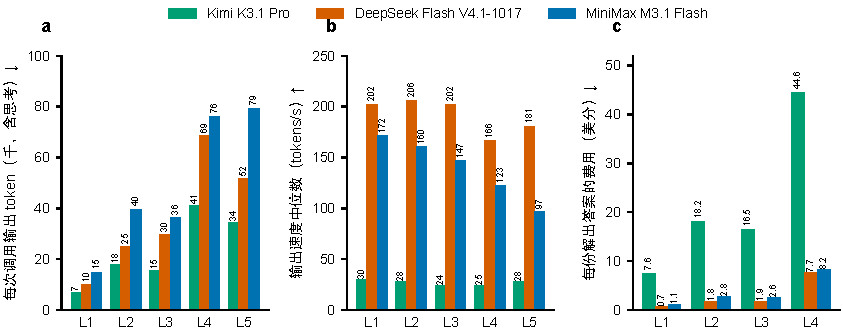
\includegraphics[width=\linewidth]{figures/fig6_cost.pdf}
  \caption{\textbf{用量、速度与费用。}(a) 每次调用的平均输出 token（含思考）；(b) 输出速度中位数；(c) 每份解出答案的费用（L1--L4）。}
  \label{fig:cost}
\end{figure}

\lead{\kimi 输出最短，但速度最慢、费用最高。}\kimi 每次调用平均输出 24.6k token，少于 \ds 的 41.2k 与 \mini 的 51.8k；但它的输出速度中位数只有每秒 25.6 token，\ds 为 195.3、\mini 为 144.8，因此延迟中位数最长（675 秒，\ds 为 162 秒，\mini 为 324 秒）。按官方美元标价，完成全部 202 个采样的费用分别为 50.12、5.79 与 6.30 美元；L1--L4 每份解出答案的费用分别为 0.244、0.033 与 0.037 美元，\kimi 约为另外两个模型的 7 倍。

\lead{\ds 与 \mini 的费用相近，原因不同。}\mini 的输出单价只有 \ds 高峰价的一半，但每次调用的输出更长，解出的题也更少；\ds 的调用多在非高峰时段，实际按半价计费。在 L4、L5 上，\mini 的输出速度降至每秒 122.8 与 97.1 token，延迟中位数分别为 526 与 790 秒。

\FloatBarrier
\section{结论}

我们提出了 codingBench 阶梯评测：以人类竞赛组别为难度标尺，从官方来源构建五档、112 道题，按官方时限判题，并与官方解比较运行效率与复杂度，同时报告输出 token、输出速度与费用。对三个模型的评测表明，\kimi 与 \ds 在 L3 上的 pass@1 都在 95\% 以上，模型之间的差距从 L4 开始拉开：\kimi 在 L4 上的 pass@1 为 92.6\%，\ds 与 \mini 为 72.2\% 与 55.6\%，三组两两差值在 L1--L4 合计上均显著。\kimi 的这一领先依赖 max 思考强度：high 下它的 L4 pass@1 为 64.8\%，低于 \ds；而 max 对开放式的 L5 没有显著作用。\kimi 的领先也以速度与费用为代价，它的输出速度不到另外两个模型的五分之一，每份解出答案的费用约为它们的 7 倍。三个模型在 L5 上都远低于官方参考解，这一档仍有很大的区分空间。后续工作包括：评测更多模型与思考强度，支持交互题与 IOI 的通信题，以及为 USACO 编写输入生成器，做真正的规模扫描。

\section*{局限性}

\begin{itemize}[leftmargin=1.6em]
  \item \lead{调用参数不对等。}\ds 使用接口默认的 high，\kimi 与 \mini 以 max 为主；采样参数也不同：\kimi 使用接口默认的 temperature 与 top\_p，\ds 在思考模式下忽略 temperature，\mini 为 0.2。
  \item \lead{L4 的 max 结果部分沿用 high 的答案。}L4 中 high 下输出正确的 36 个采样没有以 max 重新作答，max 一组对这些采样的结果等于 high。
  \item \lead{归因是观测上的一致，而非因果。}三个模型在数据、规模与训练方法上同时不同，本文既没有消融实验，也没有评测它们的前代。
  \item \lead{题目覆盖不全。}EGOI 的 2 道交互题与 IOI 2026 的题目没有纳入；高档题量少，L3、L4 只有 27 与 18 题，区间较宽。
  \item \lead{效率比较存在选择偏差。}运行效率与代码质量只比较各自解出的答案，三个模型解出的题并不相同。
  \item \lead{费用与速度依赖调用条件。}费用按公开标价计算，不代表订阅或折扣后的实际支出；输出速度受并发与网络条件影响。
\end{itemize}

\bibliographystyle{unsrtnat}
\bibliography{refs}

\appendix
\section{\kimi 逐个采样的 high 与 max 得分}
\label{app:effort}

L4 列出 high 下输出有误、以 max 作答的 18 个采样，L5 列出全部 30 题。得分按官方时限计算，变化为 max 减 high。

{\small\begin{longtable}{@{}llrrr@{}}
\toprule
采样 & 档位 & high 得分 $\uparrow$ & max 得分 $\uparrow$ & 变化 \\
\midrule\endhead
usaco-1477\#0 & L4 & 14.3 & 100.0 & +85.7 \\
usaco-1477\#2 & L4 & 14.3 & 100.0 & +85.7 \\
usaco-1500\#1 & L4 & 23.1 & 100.0 & +76.9 \\
usaco-1500\#2 & L4 & 23.1 & 100.0 & +76.9 \\
usaco-1501\#0 & L4 & 78.9 & 100.0 & +21.1 \\
usaco-1526\#2 & L4 & 5.0 & 100.0 & +95.0 \\
usaco-1548\#2 & L4 & 4.8 & 100.0 & +95.2 \\
usaco-1550\#1 & L4 & 18.2 & 100.0 & +81.8 \\
usaco-1550\#2 & L4 & 18.2 & 100.0 & +81.8 \\
usaco-1572\#0 & L4 & 18.2 & 18.2 & +0.0 \\
usaco-1572\#1 & L4 & 9.1 & 100.0 & +90.9 \\
usaco-1572\#2 & L4 & 18.2 & 18.2 & +0.0 \\
usaco-1573\#0 & L4 & 0.0 & 100.0 & +100.0 \\
usaco-1573\#1 & L4 & 0.0 & 100.0 & +100.0 \\
usaco-1573\#2 & L4 & 0.0 & 100.0 & +100.0 \\
usaco-1574\#2 & L4 & 13.0 & 100.0 & +87.0 \\
usaco-1596\#1 & L4 & 28.6 & 100.0 & +71.4 \\
usaco-1596\#2 & L4 & 61.9 & 28.6 & $-$33.3 \\
fcs-0 & L5 & 60.4 & 60.3 & $-$0.1 \\
fcs-104 & L5 & 35.3 & 0.0 & $-$35.3 \\
fcs-111 & L5 & 60.0 & 60.0 & +0.0 \\
fcs-121 & L5 & 28.1 & 19.9 & $-$8.2 \\
fcs-13 & L5 & 16.3 & 49.0 & +32.7 \\
fcs-132 & L5 & 16.8 & 32.0 & +15.2 \\
fcs-141 & L5 & 60.5 & 58.5 & $-$2.0 \\
fcs-148 & L5 & 0.0 & 0.0 & +0.0 \\
fcs-154 & L5 & 0.0 & 0.0 & +0.0 \\
fcs-160 & L5 & 12.9 & 4.1 & $-$8.7 \\
fcs-166 & L5 & 27.5 & 0.0 & $-$27.5 \\
fcs-174 & L5 & 3.3 & 3.3 & +0.0 \\
fcs-183 & L5 & 31.6 & 31.9 & +0.2 \\
fcs-193 & L5 & 60.4 & 60.4 & +0.0 \\
fcs-211 & L5 & 52.3 & 52.3 & +0.0 \\
fcs-222 & L5 & 9.3 & 9.3 & +0.0 \\
fcs-23 & L5 & 0.0 & 61.4 & +61.4 \\
fcs-239 & L5 & 45.7 & 54.9 & +9.2 \\
fcs-249 & L5 & 60.1 & 60.1 & +0.0 \\
fcs-257 & L5 & 46.3 & 38.5 & $-$7.8 \\
fcs-30 & L5 & 42.6 & 42.6 & +0.0 \\
fcs-304 & L5 & 58.5 & 58.5 & +0.0 \\
fcs-310 & L5 & 62.2 & 61.1 & $-$1.1 \\
fcs-42 & L5 & 59.3 & 59.0 & $-$0.3 \\
fcs-48 & L5 & 25.3 & 22.8 & $-$2.5 \\
fcs-58 & L5 & 33.1 & 60.1 & +27.0 \\
fcs-6 & L5 & 48.6 & 59.5 & +10.9 \\
fcs-68 & L5 & 0.0 & 60.1 & +60.1 \\
fcs-77 & L5 & 53.5 & 49.4 & $-$4.1 \\
fcs-85 & L5 & 59.8 & 0.0 & $-$59.8 \\
\bottomrule
\end{longtable}
}

\section{提示词}
\label{app:prompts}

USACO 与 EGOI 题沿用 LiveCodeBench 的写法，并给出时限与内存限制；FrontierCS 使用其官方生成脚本的原始提示词，便于与其公开排行榜对照。系统提示词与格式说明如下（原文为英文）：

{\raggedright
\begin{itemize}[leftmargin=1.6em]
  \item Python 档系统提示词：\texttt{You are an expert Python programmer. You will be given a question (problem specification) and will generate a correct Python program that matches the specification and passes all tests.}
  \item C++ 档系统提示词：\texttt{You are an expert competitive programmer. You will be given a question (problem specification) and will generate a correct and efficient C++17 program that matches the specification and passes all tests.}
  \item 用户消息：\texttt{\#\#\# Question:} 之后为题面，随后一行写明时限、内存限制与语言（如 \texttt{Time limit: 2 seconds per test. Memory limit: 256 MB. Compiled with g++ -O2 -std=gnu++17.}），再给出格式说明：\texttt{Read the inputs from stdin solve the problem and write the answer to stdout (do not directly test on the sample inputs). Enclose your code within delimiters as follows.}
  \item FrontierCS：\texttt{You are a competitive programmer. You will be given a problem statement, please implement a solution in C++. The execution time and memory limit are also stated in the statement so be aware of the complexity of the program. Please wrap the code in \textasciigrave\textasciigrave\textasciigrave cpp and \textasciigrave\textasciigrave\textasciigrave{} so that it is properly formatted. Your response should ONLY contain the C++ code, with no additional explanation or text.}
\end{itemize}
}

答案取回答中最后一个对应语言的代码块（LiveCodeBench 的规则），没有对应语言时取最后一个代码块。

\section{复现}
\label{app:repro}

代码、题单生成脚本与本文的全部图表脚本见 \url{https://github.com/BAI-AI-Lab/codingBench}。题面、测试数据与官方题解不随仓库发布，需从官方来源重新下载并建库：

{\small
\begin{verbatim}
cb ladder-data                 # 下载官方数据（可断点续传）
cb ladder-build --calibrate    # 整理题目，判官方解并选出性能对照
export MODEL=... OPENAI_BASE_URL=... OPENAI_API_KEY=... REASONING_EFFORT=...
cb ladder --smoke              # 每档 1 题，先确认接口
cb ladder                      # 生成、判题、性能复测、复杂度、静态质量、报告
\end{verbatim}
}

本文的数字、表格与图由 \texttt{collect.py}（逐个采样的得分与用量，不含题目内容）、\texttt{analysis.py}（统计量）、\texttt{make\_tables.py}（表格）与 \texttt{make\_figures.py}（绘图）生成。

\vspace{2em}\begin{flushright}由 Albert Huang 创建于 2026-11-03\end{flushright}

\end{document}
